\documentclass[11pt,a4paper]{article}
\usepackage[utf8]{inputenc}
\usepackage[T1]{fontenc}
\usepackage{geometry}
\usepackage{amsmath}
\usepackage{booktabs}
\usepackage{graphicx}
\usepackage{hyperref}
\usepackage{caption}
\usepackage{array}
\geometry{margin=2.3cm}
\setlength{\parskip}{0.65em}
\setlength{\parindent}{0pt}

% Auto-generated by scripts/run_wp1_simple_calculations.py

\newcommand{\DryAirFlow}{1}

\newcommand{\BaselineLoad}{51.31}

\newcommand{\StateTable}{%
\begin{tabular}{lrrrrr}
\toprule
State & $T$ & RH & $w$ & $h$ & $T_{dew}$ \\
\midrule
Baseline inlet: 32C, 80\% RH & 32.0 & 80 & 24.27 & 94.35 & 28.11 \\
Pre-dried: 32C, 50\% RH & 32.0 & 50 & 14.95 & 70.48 & 20.28 \\
Pre-dried: 32C, 30\% RH & 32.0 & 30 & 8.89 & 54.94 & 12.27 \\
Target: 22C, 50\% RH & 22.0 & 50 & 8.22 & 43.03 & 11.11 \\
\bottomrule
\end{tabular}
}

\newcommand{\LoadTable}{%
\begin{tabular}{lrrrrrr}
\toprule
Case & COP & $Q_{down}$ & $P_{down}$ & $P_{saved}$ & Saving & $\dot m_w$ \\
\midrule
Baseline inlet: 32C, 80\% RH & fixed\_COP\_3 & 51.31 & 17.10 & 0.00 & 0.0 & 0.00 \\
Baseline inlet: 32C, 80\% RH & fixed\_COP\_5 & 51.31 & 10.26 & 0.00 & 0.0 & 0.00 \\
Pre-dried: 32C, 50\% RH & fixed\_COP\_3 & 27.44 & 9.15 & 7.96 & 46.5 & 33.56 \\
Pre-dried: 32C, 50\% RH & fixed\_COP\_5 & 27.44 & 5.49 & 4.77 & 46.5 & 33.56 \\
Pre-dried: 32C, 30\% RH & fixed\_COP\_3 & 11.91 & 3.97 & 13.13 & 76.8 & 55.40 \\
Pre-dried: 32C, 30\% RH & fixed\_COP\_5 & 11.91 & 2.38 & 7.88 & 76.8 & 55.40 \\
\bottomrule
\end{tabular}
}

\newcommand{\ThresholdTable}{%
\begin{tabular}{lrrrr}
\toprule
Case & COP & $\dot m_w$ & $P_{saved}$ & $e_{p,max}$ \\
\midrule
Pre-dried: 32C, 50\% RH & fixed\_COP\_3 & 33.56 & 7.96 & 237 \\
Pre-dried: 32C, 50\% RH & fixed\_COP\_5 & 33.56 & 4.77 & 142 \\
Pre-dried: 32C, 30\% RH & fixed\_COP\_3 & 55.40 & 13.13 & 237 \\
Pre-dried: 32C, 30\% RH & fixed\_COP\_5 & 55.40 & 7.88 & 142 \\
\bottomrule
\end{tabular}
}

\newcommand{\GibbsTable}{%
\begin{tabular}{lrrr}
\toprule
Activity ratio & $T$ & $g_{min}$ & $g_{min}$ \\
\midrule
0.8/0.5 & 32.0 & 66.2 & 18.4 \\
0.8/0.3 & 32.0 & 138.1 & 38.4 \\
\bottomrule
\end{tabular}
}

\newcommand{\HeatTable}{%
\begin{tabular}{lrrrr}
\toprule
Case & $\dot m_w$ & $q_{sorp}$ & $Q_{sorp}$ & $P_{reject,COP3}$ \\
\midrule
Pre-dried: 32C, 50\% RH & 33.56 & 2431 & 22.66 & 7.55 \\
Pre-dried: 32C, 30\% RH & 55.40 & 2431 & 37.41 & 12.47 \\
\bottomrule
\end{tabular}
}

\newcommand{\AreaTable}{%
\begin{tabular}{lrr}
\toprule
Case & $J_w$ & $A_m$ \\
\midrule
Pre-dried: 32C, 50\% RH & 1000 & 33.56 \\
Pre-dried: 32C, 50\% RH & 3000 & 11.19 \\
Pre-dried: 32C, 50\% RH & 10000 & 3.36 \\
Pre-dried: 32C, 30\% RH & 1000 & 55.40 \\
Pre-dried: 32C, 30\% RH & 3000 & 18.47 \\
Pre-dried: 32C, 30\% RH & 10000 & 5.54 \\
\bottomrule
\end{tabular}
}

\title{WP1: Enkle termodynamiske beregninger for EO pre-drying i HVAC}
\author{HeiQ Thermodynamical Analysis}
\date{\today}

\begin{document}
\maketitle

\section{Problemstilling}

Hovedspørsmålet i WP1 er om elektro-osmotisk (EO/ACEO) pre-drying kan redusere kjøpt energi i et HVAC-system sammenlignet med vanlig avfukting med kald coil. I dette dokumentet ser vi bare på de enkle, transparente beregningene som ikke krever dynamiske simuleringer eller detaljerte membranmodeller.

Vi vurderer tre innluftstilstander ved samme tørrkuletemperatur:
\begin{align*}
    A_0 &= 32^\circ\mathrm{C},\ 80\%\mathrm{RH}, \\
    A_{50} &= 32^\circ\mathrm{C},\ 50\%\mathrm{RH}, \\
    A_{30} &= 32^\circ\mathrm{C},\ 30\%\mathrm{RH},
\end{align*}
med felles sluttpunkt
\begin{equation*}
    D = 22^\circ\mathrm{C},\ 50\%\mathrm{RH}.
\end{equation*}

Angrepsmåten er:
\begin{enumerate}
    \item Beregn fuktighetsforhold, entalpi og duggpunkt for alle relevante lufttilstander.
    \item Beregn hvor mye downstream HVAC-last reduseres dersom luften pre-tørkes fra 80\% RH til 50\% RH eller 30\% RH ved 32$^\circ$C.
    \item Oversett redusert kjølelast til redusert elektrisk effekt med faste COP-verdier 3 og 5.
    \item Beregn hvor lav EO-energi per kg vann, $e_p$, må være for at pre-drying skal lønne seg før mer detaljerte tap tas med.
    \item Beregn grove størrelsesordener for Gibbs-separasjonsarbeid, sorpsjonsvarme og membranareal.
\end{enumerate}

Alle tall i dokumentet er gitt per
\begin{equation*}
    \dot m_{da} = \DryAirFlow\ \mathrm{kg_{dry\ air}/s}.
\end{equation*}
Skalering til andre luftmengder er lineær i første orden.

\section{Psykrometriske formler}

Fuktighetsforholdet beregnes fra partialtrykket til vanndamp:
\begin{equation}
    w = 0.621945\frac{p_w}{p-p_w},
\end{equation}
der $p_w = RH\,p_{ws}(T)$ og $p$ er totaltrykket. Fuktig-luft-entalpien skrives med vanlig HVAC-referanse som
\begin{equation}
    h = 1.006T + w\left(2501 + 1.86T\right),
\end{equation}
der $T$ er i $^\circ$C, $w$ er i kg vann per kg tørrluft, og $h$ er i kJ/kg tørrluft.

Tabell~\ref{tab:states} viser tilstandene som brukes i beregningen.

\begin{table}[h!]
\centering
\caption{Psykrometriske tilstander. $w$ er i g/kg tørrluft, $h$ i kJ/kg tørrluft, og temperaturer i $^\circ$C.}
\label{tab:states}
\resizebox{\textwidth}{!}{\StateTable}
\end{table}

\begin{figure}[h!]
\centering
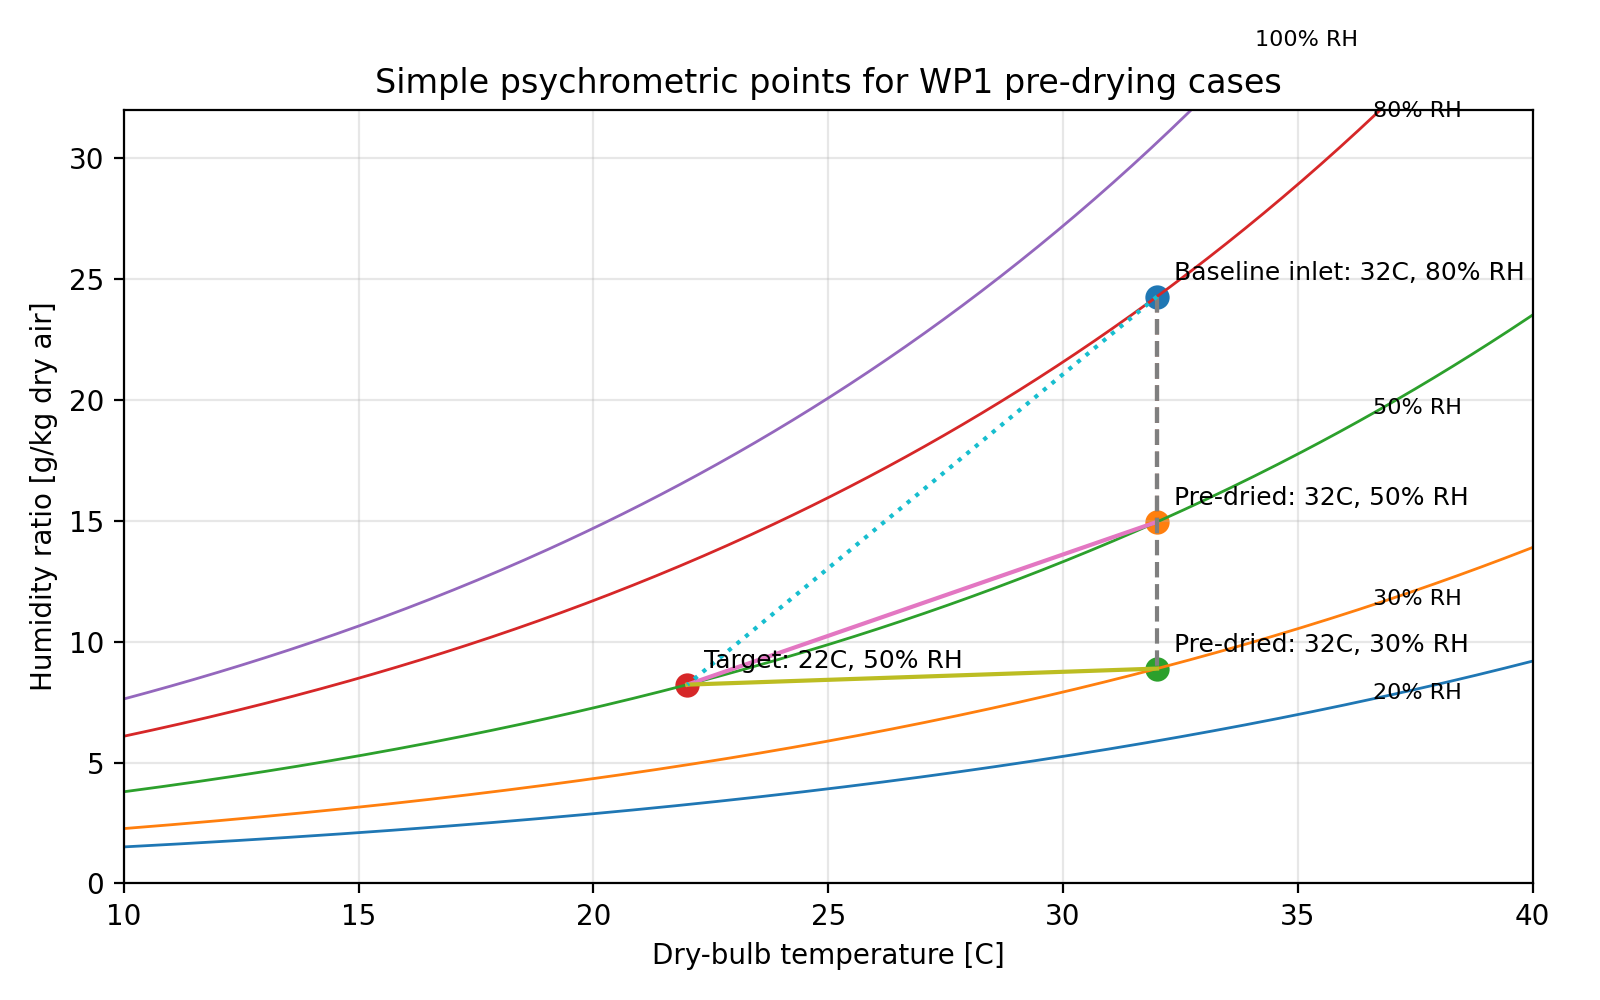
\includegraphics[width=0.86\textwidth]{figures/wp1_psychrometric_points.png}
\caption{Forenklet psykrometrisk plot med de tre starttilstandene og måltilstanden. Kurvene er RH-kurver. Figuren er ikke ment som et fullstendig ASHRAE-diagram, men som en visuell kontroll av beregningspunktene.}
\label{fig:psychrometric}
\end{figure}

\section{Redusert HVAC-last fra pre-drying}

Kjølelasten som gjenstår etter eventuell pre-drying estimeres fra entalpiforskjellen
\begin{equation}
    \dot Q_{down} = \dot m_{da}\left(h_{in}-h_D\right).
\end{equation}

Kjøpt elektrisk effekt til kjøling estimeres som
\begin{equation}
    P_{cool}=\frac{\dot Q_{down}}{COP}.
\end{equation}

Tabell~\ref{tab:load} viser direkte lastreduksjon dersom pre-drying-stegene antas å være gratis. Dette er ikke en full systemkonklusjon; det er verdien av pre-drying før EO-energi, vifter og varmehåndtering trekkes fra.

\begin{table}[h!]
\centering
\caption{Downstream kjølelast og kjøpt effekt. $Q_{down}$ og $P$ er i kW per kg tørrluft/s. $\dot m_w$ er vann fjernet i pre-drying-steget i kg/h.}
\label{tab:load}
\resizebox{\textwidth}{!}{\LoadTable}
\end{table}

\begin{figure}[h!]
\centering
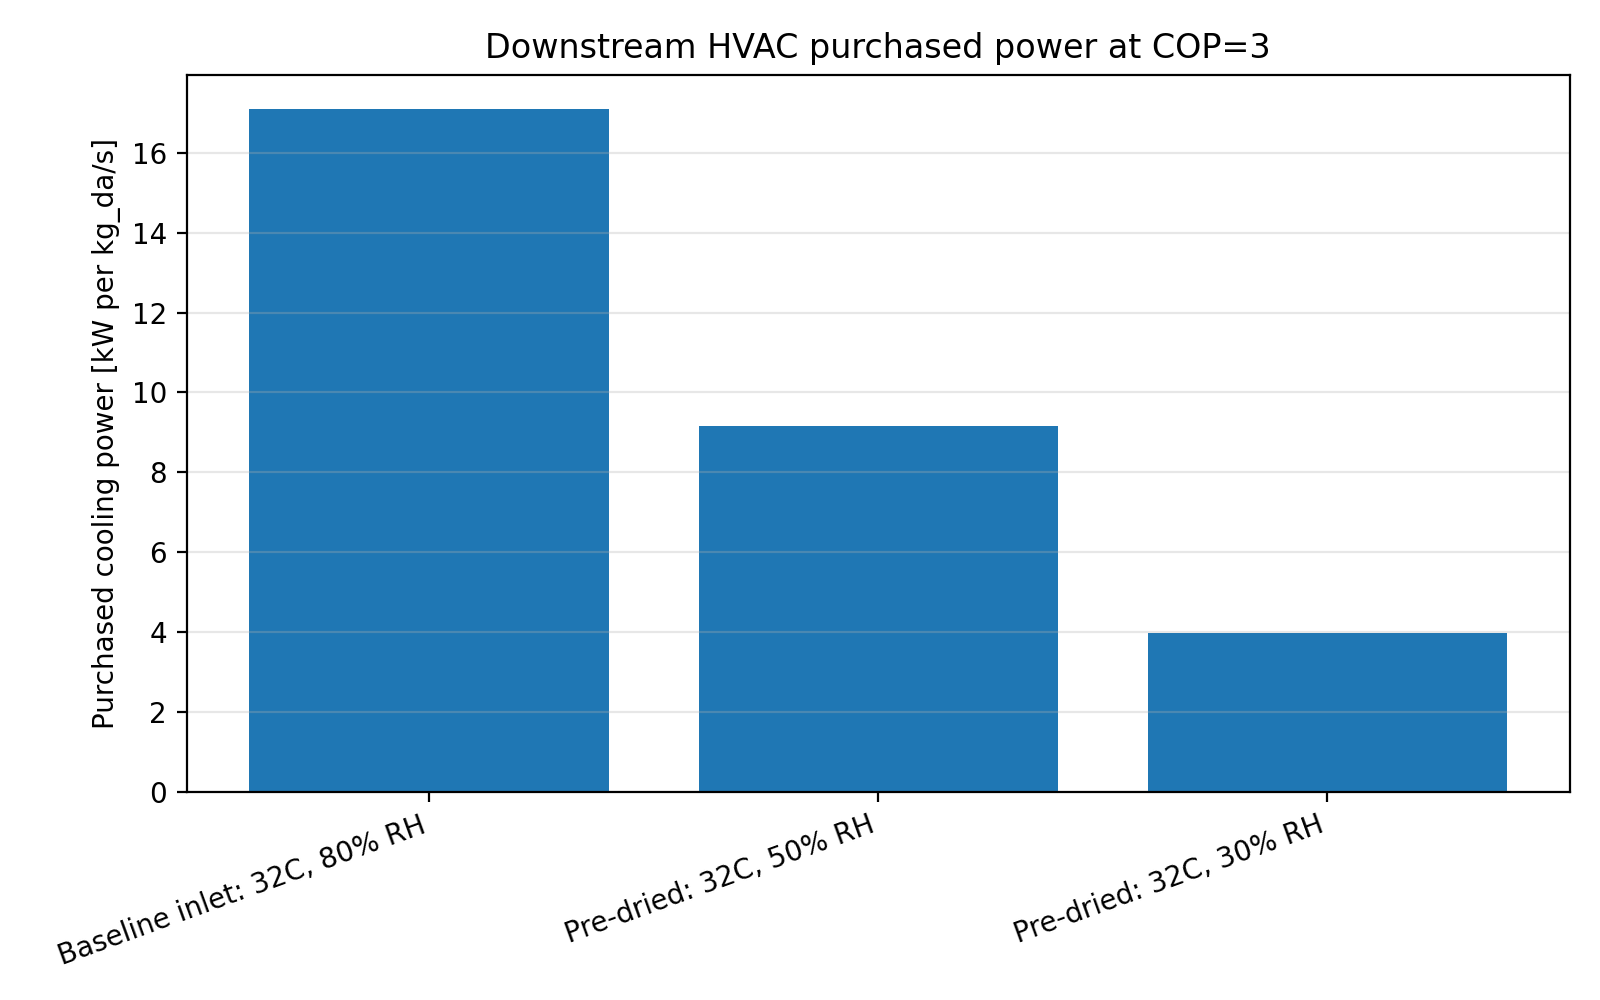
\includegraphics[width=0.82\textwidth]{figures/wp1_cooling_power_COP3.png}
\caption{Kjøpt downstream kjøleeffekt ved COP=3. Pre-drying fra 80\% til 50\% RH halverer omtrent downstream kjøpt effekt. Pre-drying til 30\% RH reduserer lasten enda mer, men krever også mer vanntransport i membranen.}
\label{fig:cooling_power}
\end{figure}

\section{Break-even EO-energi}

Dersom membranen fjerner vannmengden $\dot m_w$, og EO-energiforbruket er $e_p$ Wh/kg vann, blir EO-effekten
\begin{equation}
    P_{EO} = \dot m_w e_p,
\end{equation}
der $\dot m_w$ må uttrykkes konsistent. I SI-enheter gir
\begin{equation}
    P_{EO}\,[\mathrm{W}] = \dot m_w\,[\mathrm{kg/s}]\,e_p\,[\mathrm{Wh/kg}]\,3600.
\end{equation}

Break-even-verdien for $e_p$ er derfor
\begin{equation}
    e_{p,\max}=\frac{P_{saved}}{3600\dot m_w}.
\end{equation}
Hvis $e_p<e_{p,\max}$ kan pre-drying spare kjøpt kjøleenergi før øvrige tap tas med. Hvis $e_p>e_{p,\max}$ spiser EO-arbeidet opp gevinsten.

\begin{table}[h!]
\centering
\caption{Break-even EO-energi før varmehåndtering og vifteenergier. $e_{p,\max}$ er i Wh/kg vann.}
\label{tab:thresholds}
\resizebox{0.95\textwidth}{!}{\ThresholdTable}
\end{table}

\begin{figure}[h!]
\centering
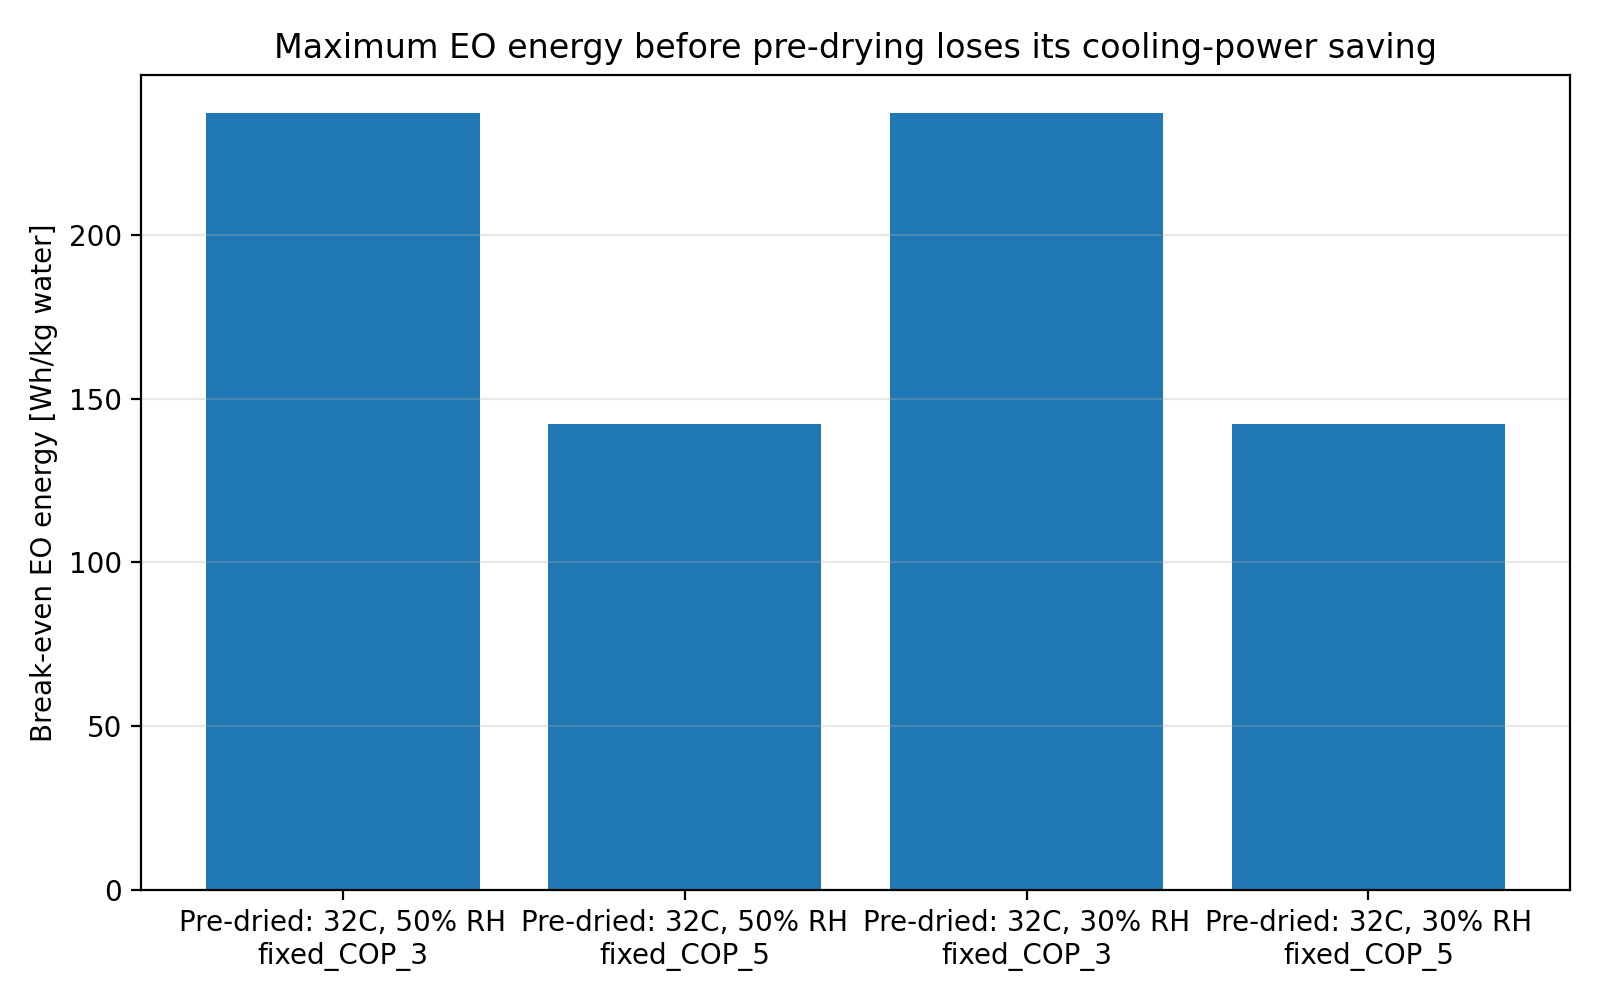
\includegraphics[width=0.78\textwidth]{figures/wp1_ep_break_even.png}
\caption{Break-even $e_p$ for faste COP-verdier. Ved COP=3 ligger break-even rundt 237 Wh/kg vann. Ved COP=5 ligger den rundt 142 Wh/kg vann. Dette er før ekstra vifte- og varmehåndteringskostnader.}
\label{fig:ep_budget}
\end{figure}

\section{Gibbs-arbeid som nedre grense}

En enkel størrelsesorden for reversibelt separasjonsarbeid kan estimeres med vannaktivitet
\begin{equation}
    g_{min} \approx R_vT\ln\left(\frac{a_{high}}{a_{low}}\right),
\end{equation}
der $a\approx RH$ for vanndamp. Dette er ikke en full prosessintegralmodell, men gir en nyttig nedre grense for hvor lavt EO-energiforbruket kan tenkes å komme.

\begin{table}[h!]
\centering
\caption{Grov Gibbs-/aktivitetsbasert energiskala. $g_{min}$ er gitt både i kJ/kg vann og Wh/kg vann.}
\label{tab:gibbs}
\GibbsTable
\end{table}

Tolkningen er at et målområde rundt 50--100 Wh/kg vann ikke bryter med enkle termodynamiske størrelsesordener, men det krever at elektroder, membran og varmehåndtering er effektive.

\section{Sorpsjonsvarme og varmehåndtering}

Hvis vann tas opp i en membran med lavere partiell entalpi enn vanndamp, forsvinner ikke entalpien. Den frigjøres som sorpsjonsvarme:
\begin{equation}
    q_{sorp}=h_v-\bar h_{w,mem}.
\end{equation}
Varmeskalaen blir
\begin{equation}
    \dot Q_{sorp}=\dot m_w q_{sorp}.
\end{equation}

Tabell~\ref{tab:heat} viser varmen som må håndteres dersom $q_{sorp}\approx 2431$ kJ/kg, omtrent latentvarmen nær romtemperatur.

\begin{table}[h!]
\centering
\caption{Sorpsjonsvarme for pre-drying-stegene ved $q_{sorp}=2431$ kJ/kg. $P_{reject,COP3}$ viser kjøpt effekt dersom all denne varmen måtte fjernes aktivt med COP=3.}
\label{tab:heat}
\resizebox{0.95\textwidth}{!}{\HeatTable}
\end{table}

\begin{figure}[h!]
\centering
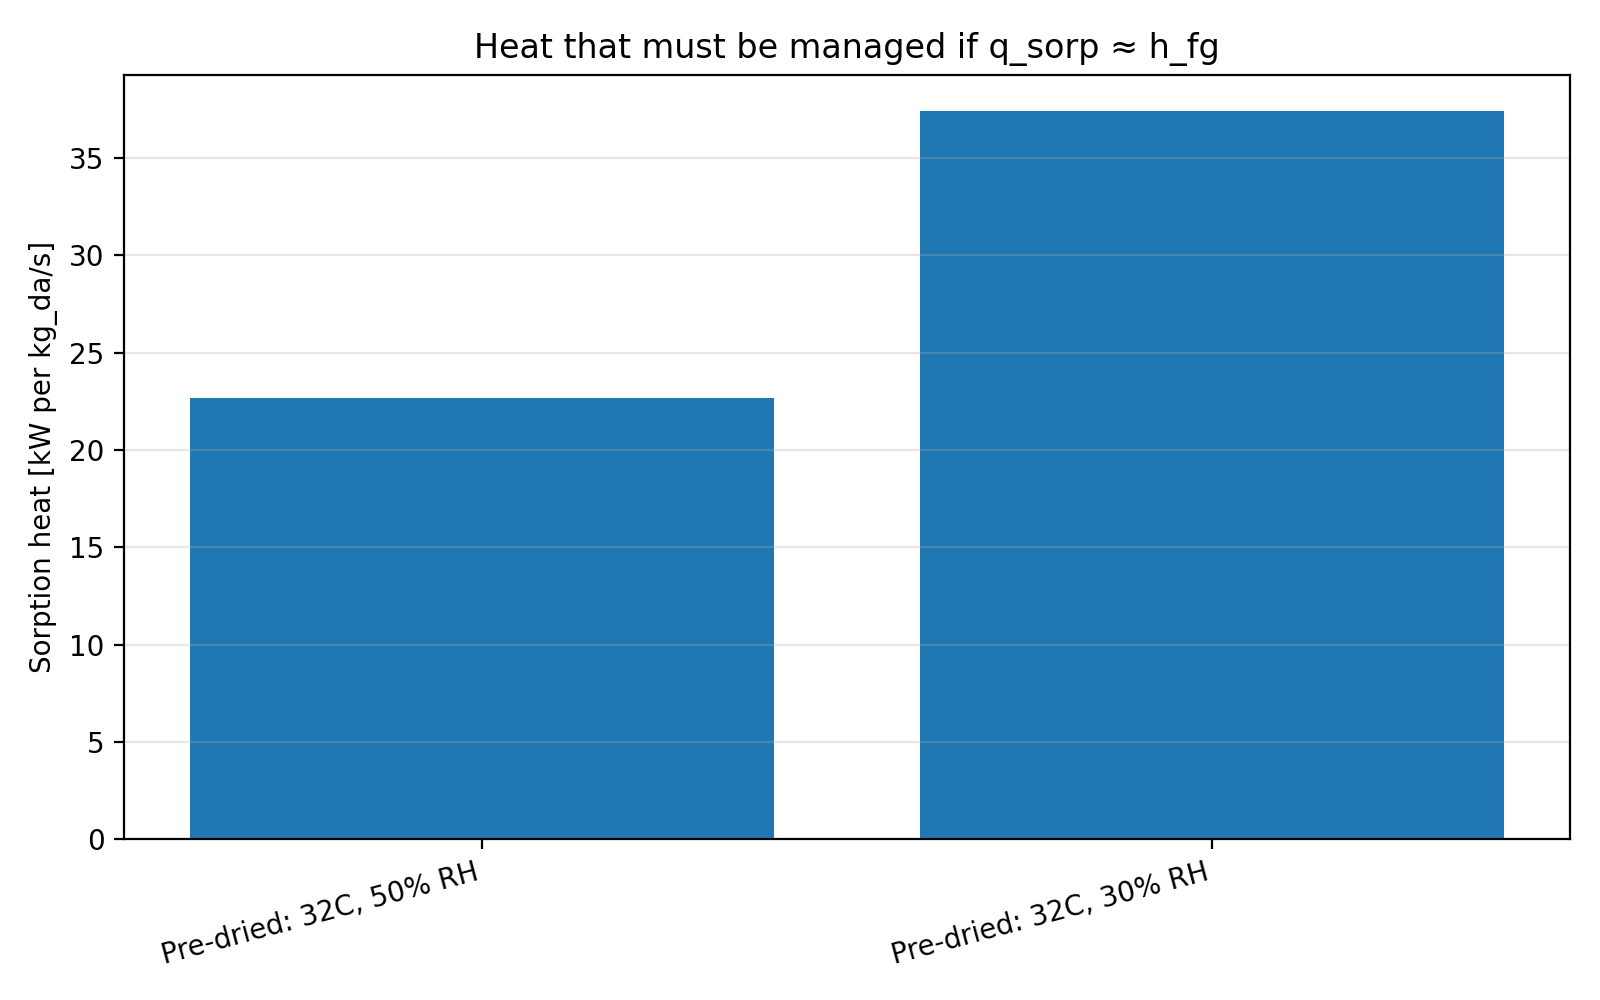
\includegraphics[width=0.80\textwidth]{figures/wp1_sorption_heat.png}
\caption{Sorpsjonsvarme som må håndteres. Denne varmen kan være større enn EO-elektrisk input, og er derfor en sentral del av WP1 selv i en enkel beregning.}
\label{fig:heat}
\end{figure}

\section{Membranareal fra enkel flux-beregning}

Hvis membranen skal fjerne $\dot m_w$ kg/h og den aktive vannfluxen er $J_w$ g/(m$^2$h), blir nødvendig aktivt membranareal
\begin{equation}
    A_m = \frac{1000\dot m_w}{J_w}.
\end{equation}

\begin{table}[h!]
\centering
\caption{Nødvendig aktivt membranareal for noen representative fluxer. $J_w$ er i g/(m$^2$h), og $A_m$ er i m$^2$.}
\label{tab:area}
\resizebox{0.85\textwidth}{!}{\AreaTable}
\end{table}

\section{Konklusjoner fra de enkle beregningene}

De enkle beregningene gir følgende foreløpige WP1-konklusjoner:

\begin{enumerate}
    \item Pre-drying fra 32$^\circ$C, 80\% RH til 32$^\circ$C, 50\% RH reduserer downstream entalpilast fra omtrent 51.3 til 27.4 kJ/kg tørrluft. Dette er en reduksjon på omtrent 46.5\%.
    \item Pre-drying til 32$^\circ$C, 30\% RH reduserer downstream entalpilast til omtrent 11.9 kJ/kg tørrluft, men krever også at membranen fjerner omtrent 55.4 kg vann/h per kg tørrluft/s.
    \item Før vifter og varmehåndtering må $e_p$ være lavere enn omtrent 237 Wh/kg vann ved COP=3, eller omtrent 142 Wh/kg vann ved COP=5, for at EO-pre-drying skal lønne seg i ren elektrisk kjøleenergi.
    \item Den aktivitetsbaserte nedre grensen er mye lavere, omtrent 18 Wh/kg for 80\% til 50\% RH og 38 Wh/kg for 80\% til 30\% RH. Det betyr at et praktisk mål på 50--100 Wh/kg er termodynamisk mulig, men ikke garantert.
    \item Sorpsjonsvarmen er stor: omtrent 22.7 kW for 80\% til 50\% RH og 37.4 kW for 80\% til 30\% RH ved $\dot m_{da}=1$ kg/s. Hvis denne varmen går tilbake til prosessluften eller må fjernes aktivt, kan gevinsten reduseres kraftig.
    \item Arealkravet er sterkt flux-avhengig. For 32$^\circ$C, 80\% til 50\% RH trengs omtrent 11.2 m$^2$ ved 3000 g/(m$^2$h), men 33.6 m$^2$ ved 1000 g/(m$^2$h).
\end{enumerate}

Stage-gate-spørsmålet bør derfor formuleres som:
\begin{equation*}
    \boxed{e_p,\ J_w,\ A_m\ \text{og varmehåndtering må samtidig være gode nok.}}
\end{equation*}
Lavt $e_p$ alene er ikke tilstrekkelig dersom sorpsjonsvarmen ikke kan avvises gunstig eller dersom membranarealet blir for stort.

\section{Hvordan tallene kan regenereres}

Tallene og figurene i dette dokumentet kan genereres med:
\begin{verbatim}
python scripts/run_wp1_simple_calculations.py \
  --out outputs/wp1_simple_calculations
\end{verbatim}

For et annet sluttpunkt, for eksempel 20$^\circ$C og 50\% RH, kan man bruke:
\begin{verbatim}
python scripts/run_wp1_simple_calculations.py \
  --out outputs/wp1_simple_calculations_20C \
  --target-T-C 20 \
  --target-RH 0.50
\end{verbatim}

\end{document}
